%%%%%%%%%%%%%%%%%%%%%%%%%%%%%%%%%%%%%%%%%%%%%%%%%%%%%%%%%%%%%%%%%%%%%%%%%%%%%%%%%%%
%%Anna University sample latex thesis format for UG thesis
%--------------------------------
%%This is the main file that includes the front matter and other chapter links. 
%%Chapters are placed within the folder named 1, 2,...  
%%To compile, run the command `pdflatex authesis.tex' in the terminal. 
%%Some packages may not be needed. Comment the ones, that are not needed. 
%%Images can be saved in the format of *.png. 
%%------------------------------------------------------
%% Authors:
%%Originally used by Dr. Mary Anita Rajam and then modified by Dr. Bama Srinivasan according to the latest Anna University regulations. %%Please report changes to bama@annauniv.edu, chorse@gmail.com %%
%%Acknowledgement: Thanks to Dr.Ranjani Parthasarathi, who relentlessly and patiently guided Bama Srinivasan.
%---------------------------------------------------------
%% Modification added:
%%new file apalikem is added, which gives a neat reference list with 1, 2...
%%aureportm has appendix starting with Arabic numbers
%% Disclaimer: Check with the latest Anna University regulations before working with this format.
%% Changes as on July 2016 
%% 1. Changed the appendix back to alpha mode in aureport.cls
%% 2. Table of contents - reduced the top margin and spacing
%% 3. Added the counter depth for sections to 4 in aureport.cls
%% 4. Deleted chapter number, title and page number in TOC
%% 5. Reduced the top space in chapter titles from 6.5 cms to 5.5 cms in aureport.cls
%% 6. Changes in references use the package natbib and style unsrt. Include a .bib file for the bibliography
%$$$$$$$$$$$$$$$$$$$$$$$$$$$$$$$$$$$$$$$$$$$$$$$$$$$$$$$$$$$$$$$$$$$$$$$$$$$$$$$$$$$$$$$$$$

\documentclass[13 pt,a4paper]{aureportm}
\usepackage{mathptm}\usepackage{etex}
\reserveinserts{28}
\renewcommand{\normalsize}{\fontsize{13 pt}{14.6 pt}\selectfont}
%\usepackage{aunatbib}
%\usepackage{apalikem}
\usepackage{natbib}
\usepackage{bussproofs} % for deduction rules 
\usepackage{auphd}
\usepackage{array}
\usepackage{tabularx}
\usepackage[none]{hyphenat}
\usepackage[chapter]{algorithm}
\usepackage{algpseudocode}
\usepackage{multirow}
\usepackage{multicol}
\usepackage{float}
\usepackage{booktabs}
\usepackage{amsmath}
\usepackage{amssymb}
\usepackage{amsthm}
\usepackage{latexsym}
\usepackage{verbatim}
\usepackage{ifthen}
\usepackage{graphicx}
\usepackage{hyperref}
\usepackage{epsfig}
\usepackage{pslatex}
\usepackage{setspace}
\usepackage{titlesec}
\usepackage[subfigure]{tocloft}
\usepackage{subfigure}
\usepackage{longtable}
\usepackage{enumerate}
\usepackage{lscape}

\usepackage[format=hang,labelfont=bf,textfont=bf]{caption}
\PassOptionsToPackage{linktocpage}{hyperref}
\tocloftpagestyle{myheadings}
\newcommand{\PreserveBackslash}[1]{\let\temp=\\#1\let\\=\temp}
\let\PBS=\PreserveBackslash

\usepackage{colortbl}
\usepackage{newlfont}


\newboolean{psoutput}
\setboolean{psoutput}{true}
\usepackage{pst-all}
\newcommand{\defname}[1]{\emph{#1}.}

\newtheorem{fact}{Fact}[chapter]

\floatstyle{ruled}
\newfloat{algorithm}{htp}{loa}
\floatname{algorithm}{Algorithm}


\titleformat{\section}[hang]{\bfseries}{\makebox[20mm][l]{\thesection}}{0pt}{}{}
\titleformat{\subsection}[hang]{\bfseries}{\makebox[20mm][l]{\thesubsection}}{0pt}{}{}



 \newcounter {definition}[chapter]
\renewcommand \thedefinition {\arabic{chapter}.\arabic{definition}}
\newenvironment{definition}
{ \refstepcounter{definition}
   {\noindent \bf Definition \arabic{chapter}.\arabic{definition}.}}
 {}
 \def\enddefinition{$\Box$}

 \newcounter {example}[chapter]
 \renewcommand \theexample
 {\arabic{chapter}.\arabic{example}}
 \newenvironment{example}
 { \refstepcounter{example}
   {\noindent \bf Example \arabic{chapter}.\arabic{example}.}}
 {}
 \def\endexample{$\Box$}

 \newcounter {proposition}[chapter]
 \renewcommand \theproposition {\arabic{chapter}.\arabic{proposition}}
 \newenvironment{proposition}
 {\refstepcounter{proposition}
   {\noindent \bf Proposition \arabic{chapter}.\arabic{proposition}. }}
 {}
 \def\endproposition{$\Box$}

\pagenumbering{roman}
\setcounter{page}{3}
%\setcounter{secnumdepth}{3}
\renewcommand{\baselinestretch}{1.5}
\newcommand{\row}{i}
\newcommand {\combined} {{C}}
\newcommand {\mtis} {}

\newboolean{showalter}
\setboolean{showalter}{true}
\newcommand{\alter}[1]{\ifthenelse{\boolean{showalter}}{ \{ #1 \} }{}}
\providecommand{\tabularnewline}{\\}
\newcommand{\bigsize}{\fontsize{15pt}{20pt}\selectfont}

\author{Author of the thesis}


\renewcommand{\cfttoctitlefont}{\bfseries\Large}
\renewcommand{\cftlottitlefont}{\bfseries\Large}
\renewcommand{\cftloftitlefont}{\bfseries\Large}


%\cftsetindents{chapter}{0mm}{10mm}
%\cftsetindents{section}{10mm}{10mm}
%\cftsetindents{subsection}{20mm}{10mm}
%\setlength{\cftbeforechapskip}{1.2\baselineskip}
%\setlength{\cftbeforesecskip}{.8\baselineskip}
%\setlength{\cftbeforesubsecskip}{.8\baselineskip}
%\setlength{\cftbeforefigskip}{.8\baselineskip}
%\setlength{\cftbeforetabskip}{.8\baselineskip}
%
\makeatletter
\renewcommand{\@dotsep}{10}
\makeatother
\renewcommand{\cftdot}{ }
\cftsetrmarg{1.2in} % changed by bama - earlier it was 1.5 inch. right margin is decreased to 1 inch.

\titleformat{\section}[hang]{\bfseries}{\makebox[20mm][l]{\thesection}}{0pt}{}{}
\titleformat{\subsection}[hang]{\bfseries}{{\thesubsection}}{0pt}{}{}
\titleformat{\subsubsection}[hang]{\normalsize\bfseries}{\makebox[20mm][l]{\thesubsubsection}}{0pt}{}{}
\titleformat{\paragraph}[hang]{\normalsize\bfseries}{\makebox[20mm][l]{\theparagraph}}{0pt}{}{}
\titleformat{\subparagraph}[hang]{\normalsize\bfseries}{\makebox[20mm][l]{\thesubparagraph}}{0pt}{}{}

\begin{document}

\pagenumbering{roman}


\thispagestyle{empty}
\begin{center}
  \LARGE
  \textbf{\uppercase{Title of Project Report}} \\
  \vspace{0.6\baselineskip}
  \bigsize{\textbf{A PROJECT REPORT}}\\
 \vspace{0.4\baselineskip}

  \normalsize{\textit{\textbf{Submitted by}}}\\
  \vspace{0.5\baselineskip}
  {
  \Large \textbf{CANDIDATE1 Roll number}}\\
  %\normalsize{\textbf{(Roll number)}}\\
  \Large{\textbf{CANDIDATE 2 Roll number}}\\
  \Large{\textbf{CANDIDATE 3 Roll number}} \\
   \vspace{0.6\baselineskip}
  %\normalsize{\textit{A report for the phase-I of the project}}\\
  \vspace{-0.1\baselineskip}
  \normalsize{\textit{submitted to the Faculty of}} \\
  \vspace{0.5\baselineskip}
  \normalsize{\textbf{INFORMATION AND COMMUNICATION ENGINEERING}} \\  
  \vspace{1\baselineskip}
  \normalsize{\textit{in partial fulfillment  for the award of the degree}}\\
  \normalsize{\textit{\textbf{of}}}\\
\vspace{.2\baselineskip}
  \bigsize{{\textbf{BACHELOR OF TECHNOLOGY}}}\\
  \normalsize{\textit{\textbf{in}}}\\
  \bigsize{{\textbf{INFORMATION TECHNOLOGY}}}\\
\end{center}
  \begin{center}
   %
\includegraphics[width=26mm,height=25mm]{auemblem.pdf}   \\
   
\includegraphics[scale=0.7]{auemblem.pdf} \\
  \normalsize{ \textbf{DEPARTMENT OF INFORMATION SCIENCE AND TECHNOLOGY }}\\
  \normalsize{\textbf{COLLEGE OF ENGINEERING, GUINDY}}\\
  \normalsize{\textbf{ANNA UNIVERSITY}}\\
  \normalsize{\textbf{CHENNAI  600 025}}\\
  \vspace{0.5\baselineskip}
  \normalsize{\textbf{MONTH YEAR }}
 \end{center}
\pagebreak

\chapter*{ANNA UNIVERSITY\\
CHENNAI - 600 025\\
%\vspace{\baselineskip}
BONA FIDE CERTIFICATE}
\newlength{\aulength}
\settowidth{\aulength}{Anna University
  Chennai}
\newlength{\datewidth}
\settowidth{\datewidth}{Chennai 600 025}

\begin{spacing}{1.5}
  \begin{sloppypar}
  \fontsize{13}{14.5}\selectfont Certified that this project report titled TITLE OF THE PROJECT TITLE OF THE PROJECT TITLE OF THE PROJECT TITLE OF THE PROJECT TITLE OF THE PROJECT is the bona fide work of NAME OF THE CANDIDATE(S) who carried out project work under my supervision. Certified further that to the best of my knowledge and belief, the work reported herein does not form part of any other thesis or dissertation on the basis of which a degree or an award was conferred on an earlier occasion on this or any other candidate.
  \end{sloppypar}
\end{spacing}
\vspace{-0.3 cm}
\begin{flushleft}
 \parbox[t]{\datewidth}{\small{\textbf{PLACE: }}\\
 \small{\textbf{DATE: }}}
 \hfill
 \parbox[t]{6 cm}{\small{\textbf{$<$NAME OF GUIDE$>$}} \\
 \small{\textbf{$<$DESIGNATION$>$}}\\
 \small{\textbf{PROJECT GUIDE}}\\
 \small{\textbf{DEPARTMENT OF IST, CEG}}\\
 \small{\textbf{ANNA UNIVERSITY}}   \\
 \small{\textbf{CHENNAI  600025}}
 }
\end{flushleft}
%\vspace{0.5 cm}
\begin{center}
 \small{\textbf{COUNTERSIGNED}}\\ 
  \vspace{1.5 cm}
  \textbf{\small{Dr. SASWATI MUKHERJEE}}\\ 
  \small{\textbf{HEAD OF THE DEPARTMENT}}\\
 \small{\textbf{DEPARTMENT OF INFORMATION SCIENCE AND TECHNOLOGY}}\\
 \small{\textbf{COLLEGE OF ENGINEERING, GUINDY}}\\
 \small{\textbf{ANNA UNIVERSITY}}   \\
 \small{\textbf{CHENNAI  600025}}
 
\end{center}



%\addtocontents{toc}{\protect\flushleft \protect\bfseries
%CHAPTER NO. \hfill TITLE \hfill PAGE NO.\endgraf}

%\addtocontents{toc}{\protect\raggedleft Page\\}

 %\addtocontents{lof}{\protect\flushleft
%\protect\bfseries FIGURE NO. \hfill
% TITLE \hfill  PAGE NO.\endgraf}%
%\addtocontents{lot}{\protect\flushleft \protect\bfseries TABLE NO. \hfill
%  TITLE \hfill  PAGE NO.\endgraf}%


\chapter*{\uppercase{ABSTRACT}}
\addcontentsline{toc}{section}{\bfseries \uppercase{Abstract}}
The abstract shall be typed in one and a half line spacing using Font Style Times New Roman and Font Size 13. This is a sample abstract in LaTeX.


\chapter*{\uppercase{ACKNOWLEDGEMENT}}
%\addcontentsline{toc}{section}{\bfseries \uppercase{Acknowledgement}}
Acknowledgement should be brief and should not exceed one page when typed in one and a half line spacing.

\setlength\cftparskip{0pt}
\setlength{\cftbeforetoctitleskip}{-3em} %Decrease the top margin of toc title
%\setlength{\cftaftertoctitleskip}{0 em} 
\setlength{\cftbeforelottitleskip}{-3em} % Decrease the top margin of lot
\setlength{\cftbeforeloftitleskip}{-3em} % Decrease the top margin of lof
\cftsetindents{chapter}{0 mm}{10 mm}
\cftsetindents{section}{10 mm}{10 mm}
\cftsetindents{subsection}{20 mm}{10 mm}
\cftsetindents{subsubsection}{30 mm}{15 mm}
\cftsetindents{paragraph}{40 mm}{20 mm}
\cftsetindents{subparagraph}{50 mm} {20  mm}
\cftsetindents{table}{10 mm}{10 mm}
\cftsetindents{figure}{10 mm}{10 mm}
%%%%%%%%%%%%%%%%%%%%%%%%%%%%%%%%%%%%%%%%%%%%%%%
%Changes made as on June 2016
%%%%%%%%ADD TOC with one half spacing%%%%%%%%%%%
\begin{onehalfspacing} 
\tableofcontents

\pagebreak

\addcontentsline{toc}{section}{\bfseries LIST OF TABLES}
\listoftables

 \clearpage \addcontentsline{toc}{section}{\bfseries
LIST OF FIGURES} \listoffigures
%\clearpage
\end{onehalfspacing}
%%%%%%%%%%%%%%%%%%%%%%%%%%%%%%%%%%%%%%%%%%%%%%
% These are old as of April 2016 -
%%%%%%%%%%%%%%%%%%%%%%%%%%%%%%%%%%%%%%%%%%%%%%%%
%\cftsetindents{chapter}{0.2in}{1.5in}
%\cftsetindents{section}{1.7in}{0.3in}
%\cftsetindents{subsection}{1.8in}{0.4in}
%\cftsetindents{table}{0.2in}{1.5in}
%\cftsetindents{figure}{0.2in}{1.5in}
%\tableofcontents



%\pagebreak

%\addcontentsline{toc}{section}{\bfseries LIST OF TABLES}
%\listoftables
% \clearpage \addcontentsline{toc}{section}{\bfseries
%LIST OF FIGURES} \listoffigures
%\clearpage
%%%%%%%%%%%%%%%%%%%%%%%%%%%%%%%%%%%%%%%%%%%%%%%%%%%%%%%%%%%
\chapter*{LIST OF SYMBOLS AND ABBREVIATIONS}
\addcontentsline{toc}{section}{\bfseries LIST OF SYMBOLS AND ABBREVIATIONS}

\setlongtables
\begin{longtable}
  {>{\PBS\raggedright\hspace{0pt}}p{3cm}@{}%
    >{\PBS\raggedright\hspace{0pt}}p{11.5cm}@{}}

  %$A$ & Set of attributes\\ 
  %$a_t$ & Time attribute\\
  $-$, $\neg$, $\sim$  & Negation operator \\
  $+$, $\vee$, $\cup$ & Disjunction operator \\
  $X$, $\wedge$ & Conjunction operator \\
  $\rightarrow$ & Conditional operator \\
  $\leftrightarrow$ & Biconditional operator \\
  $\diamond$ & Future tense modal operator\\
  $\alpha$ & Action \\    
  \end{longtable}
%\end{tabular}

%\clearpage

%\newpage
\pagenumbering{arabic}

\ausection
% Chapter 1

\chapter{\uppercase{Introduction}} % Main chapter title
\label{intro} % For referencing
This chapter is about the introduction of your project work. 
\section{\uppercase{Format of the thesis}}
A few guidelines for writing the thesis are given below. These are taken from Ph.d regulations of Anna University \cite{regulations}.
\subsection{Table of Contents}
The Table of contents should list all captions following it as well as any caption which precedes it. The title page, Certificate and Acknowledgment will not find a place among the items listed in the Table of Contents but the page numbers of which are in lower case Roman letters. One and a half line spacing should be adopted.
\subsection{List of Tables and Figures}
The list should use exactly the same captions as they appear above the Tables and Figures in the text. One and a half line spacing should be adopted.
\newpage
\subsection{List of Symbols and Abbreviations}
One and a half line spacing should be adopted for typing the matter under this head. Standard symbols, abbreviations, etc.
should be used.
\subsection{Chapters}
The chapters may be broadly divided into 3 parts (i) Introductory chapter, (ii) Chapters developing the main theme of the Thesis and (iii) Results, Discussion and Conclusion. The main text shall be divided into several chapters and each chapter may be further divided into several divisions and sub-divisions.
\begin{itemize}
 \item Each chapter should be given an appropriate title.
 \item Tables and Figures in a chapter should be placed in the immediate vicinity of the reference where they are cited.
 \item Footnotes should be used sparingly. They should be typed single space and
placed directly underneath in the very same page which refers to the material
they annotate.
\end{itemize}
\subsection{Appendices}
Appendices are provided to give supplementary information, which if included in the main text may serve as a distraction and cloud the central theme under discussion.
\begin{itemize}
 \item Appendices should be named alphabetically starting from Appendix A, Appendix B, etc.
\item  Appendices, Tables and references appearing in appendices should be numbered and referred to at appropriate places just as in the case of chapters.
\item Appendices shall carry the title of the work reported and the same title shall be included in the Table of Contents page.
\end{itemize}
\subsection{References}
Any works of other researchers, if used either directly or indirectly, the origin of the material thus referred to at appropriate places in the thesis should be indicated. Use of bibtex is recommended.
\subsection{Citation}
A few examples for citing articles, books and websites are given in Chapter \ref{ch:survey}.
\subsection{Tables and Figures}
A Table or Figure including caption should be accommodated within the prescribed margin limits and appear on the page following the page where their first reference is made.
\begin{itemize}
 \item Tables and Figures on half page or less in length may appear on the same page along with the text. However, they should be separated from the text both above and below by triple spacing.
\item Tables and Figures on half page or less in length may appear on the same page along with the text. However, they should be separated from the text both above and below by triple spacing.
\item All Tables and Figures should be prepared on the same paper or material used for the preparation of the rest of the Thesis.
\item Two or more small Tables or Figures may be grouped if necessary in a single page.
\end{itemize}
\section{\uppercase{Typing Instructions}}
Some guidelines for typing are provided below.
\subsection{General}
One and a half line spacing should be used for typing the general text. The general text shall be typed in Font Style Times New Roman and Font Size 13.
\subsection{Chapter}
The word CHAPTER without punctuation should be centered 50 mm down from the top of the page. Two spaces below, the title of the chapter should be typed centrally in capital letters. The text should commence 4 spaces below this title, the first letter of the text starting 20 mm inside from the left hand margin. The division and sub-division captions along with their numberings should be left justified. The typed material directly below division or sub-division heading should commence 2 spaces below it and should be offset 20 mm from the left hand margin. Within a division or sub-division paragraphs are permitted. Even paragraph should commence 3 spaces below the last line of the preceding paragraph, the first letter in the paragraph being offset from the left hand margin by 20 mm.
\section{\uppercase{NUMBERING INSTRUCTIONS}}
\subsection{Page Numbering}
All page numbers (whether it be in Roman or Arabic numbers) should be typed without punctuation on the upper right hand corner 20 mm from the top with the last digit in line with the right hand margin. The preliminary pages of the Thesis (such as Title page, Acknowledgement, Table of Contents, etc.) should be numbered in lower case Roman numerals. The title page will be numbered as (i) but this should not be typed. The page immediately following the title page shall be numbered as (ii) and it should appear at the top right hand corner as already specified. Pages of main text, starting with Chapter 1 should be consecutively numbered using Arabic numerals.
\subsection{Numbering of Chapters, Divisions and Subdivisions}
The numbering of chapters, divisions and sub-divisions should be done using Arabic numerals only and further decimal notation should be used for numbering the divisions and sub-divisions within a chapter. For example sub-division 4 under division 3 belonging to chapter 2 should be numbered as 2.3.4. The caption for the sub-division should immediately follow the number assigned to it. Refer below to the subsection and subsubsections. Every chapter beginning with the first chapter should be serially numbered using Arabic numerals.
\subsubsection{A subdivision of the subsection}
Use \texttt{subsubsubsection} in Latex to indicate a subdivision. The numbering should automatically appear in the Table of Contents.
\subsection{Numbering of Tables and Figures}
Tables and Figures appearing anywhere in the Thesis should bear appropriate numbers. The rule for assigning such numbers is illustrated by an example. Thus, if a Figure in Chapter 3, happens to be the fourth then assign 3.4 to that Figure. Identical rules apply for Tables except that the word Figure is replaced by the word Table. If Figures (or Tables) appear in appendices then Figure 3 in Appendix Section 2 will be designated as Figure A 2.3. If a table to be continued into the next page this may be done, but no line should be drawn underneath an unfinished Table. The top line of the Table continued into the next page should, for example read Table 2.1
(continued) placed centrally and underlined.

\subsection{Numbering of Equations}
Equations appearing in each Chapter or Appendix should be numbered serially, the numbering should commence afresh for each Chapter or Appendix.

% Chapter 2

\chapter{\uppercase{Literature Survey/Related Work}} % Main chapter title
\label{ch:survey} % For referencing

This chapter should provide the details about the related work. Atleast 20 articles should be referred and cited. The explanation should be provided within sections and subsections. 

Include the limitations of the existing work and briefly explain how your idea is advantageous over the existing ones in this chapter.
\section{\uppercase{Method of Citation}}
Following are a few methods of citation.
\subsection{Approach of Waldron}
An improved algorithm has been adopted in the literature \cite{factors}. 

\subsection{Approach by Conley}
A theory \cite{conley} on structures discusses the advantages and disadvantages. 

\subsection{Another approach}
The problem of mechanical manipulators has been studied extensively in the theory of mechanics and machines \cite{holt} and \cite{waldron}.

\section{\uppercase{Section 2}}

\subsection{Subsection 1}

\subsection{Subsection 2}

\section{\uppercase{Section 3}}

\subsection{Subsection 1}

\subsection{Subsection 2}
% Chapter 3

\chapter{\uppercase{Your work based title}} % Main chapter title
\label{ch:chap3} % For referencing
Your actual work should come in here. Include system architecture, modules, etc., with diagrams and provide an explanation for each of these. 
\section{\uppercase{View of Tables}}
Sample view  is shown in Table \ref{tab:first} and an example is given in Table~\ref{tab:second}.
\begin{table}[h]
\caption{Example 1}
\begin{center}
\begin{tabular}{|c|c|}
\hline
$c1$ & $c2$ \\
\hline
r1 & r2 \\
\hline
r1  & r2 \\
\hline
\end{tabular}
\end{center}
\label{tab:first}
\end{table}
\begin{table}[h]
\caption{Example 2}
\begin{center}
\begin{tabular}{|c|c|}
\hline
\textit{x} & \textit{y}  \\
\hline
\textit{x} & \textit{not y}  \\
\hline
\end{tabular}
\end{center}
\label{tab:second}
\end{table}

\section{\uppercase{View of Figures}}
Examples of pictures are shown in Figure \ref{fig:one} and Figure \ref{fig:two}.
\begin{figure}[h]
\begin{center}
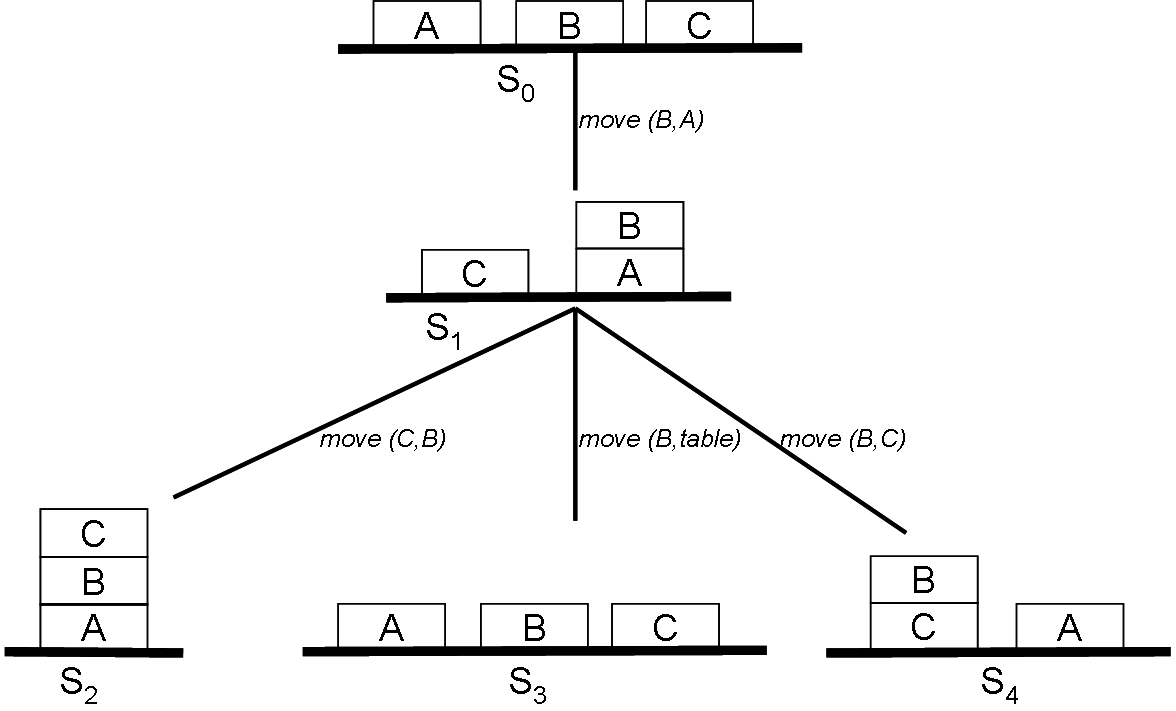
\includegraphics[scale=0.6]{3/eg1.png}
\caption{Example 1}
\label{fig:one}
\end{center}
\end{figure}
\begin{figure}[h]
\begin{center}
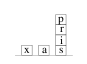
\includegraphics[scale=2]{3/eg2.png}
\caption{Example 2}
\label{fig:two}
\end{center}
\end{figure}

\section{\uppercase{View of Equations}}
The sum of squares of $a$ and $b$ are calculated as shown below:
\begin{eqnarray}
 \label{eq:sum}
 (a+b)^2 = a^2+b^2+2ab
\end{eqnarray}

From Equation \ref{eq:sum}, the data is obtained.






% Chapter 4

\chapter{\uppercase{Implementation of your work}} % Main chapter title
\label{chap4} % For referencing
The implementation details of your work should be mentioned in this chapter.
\section{\uppercase{Algorithm 1}}
\begin{algorithm}
\begin{algorithmic}[1]
\State Get the number of variables $num$ 
\State Start with an empty list $x$ $[~]$
\For {each $n$ of $num$}
	\State Get the $x$
	\State  Get the $t$
	\State Get the $w$
\EndFor 
\If {$xl$ == $s$} 
	\State terminate with the failure message \textbf{failed}
\Else
	\State $z = x$
\EndIf 

\end{algorithmic}
\end{algorithm}




% Chapter 5

\chapter{\uppercase{Implementation/ Results and Analysis}} % Main chapter title
\label{chap5} % For referencing
This chapter should provide implementation details of your work with results and analysis. 
%% Chapter 6

\chapter{\uppercase{Comparison}} % Main chapter title
\label{chap6} % For referencing
This chapter is optional. Depending on the work, comparison can also be included in previous chapter.


\chapter{\uppercase{Conclusion and Future Work}}
\label{chap:conclusion}
Conclude your work and provide an explanation for future enhancements.
\cleardoublepage
\phantomsection 
\appendix
\addcontentsline{toc}{chapter}{APPENDIX}
\chapter{\uppercase{Topic 1}}
\section{\uppercase{Section 1}}
\section{\uppercase{Section 2}}
\chapter{\uppercase{Topic 2}}
\section{\uppercase{Section 1}}
\section{\uppercase{Section 2}}






%\bibliographystyle{auapalike}
\bibliographystyle{unsrt}
\nocite{*}%This gives a list of all references that includes without citation. Remove this, once the reference is cited
\phantomsection
\addcontentsline{toc}{chapter}{REFERENCES}
\begin{spacing}{1}
\bibliography{publication}
\end{spacing}

\newpage
\clearpage




\addtocontents{toc}{\protect\newpage}
\addtocontents{lot}{\protect\newpage}
\addtocontents{lof}{\protect\newpage}

\end{document}
